\section{Desafio}

\begin{minipage}{\linewidth}
  \centering
  \begin{minipage}{0.45\linewidth}
    Dado o circuito da \textbf{Figura \ref{fig:CircuitoDesafio}},
    considerar: $R_1 = 330\Omega$,
                $R_2 = 150\Omega$,
                $R_3 = 270\Omega$, \\
                $R_4 = 400\Omega$,
                $R_5 = 100\Omega$ e
                $V_{CC} = 10V$.
    \begin{itemize}
      \item Calcular a intensidade da corrente em cada resistor;
      \item Calcular a queda de tensão em cada resistor;
    \end{itemize}
  \end{minipage}
  \hspace{0.05\linewidth}
  \begin{minipage}{0.45\linewidth}
    \begin{figure}[H]
      \centering
      \caption{Circuito elétrico misto}
      \label{fig:CircuitoDesafio}
      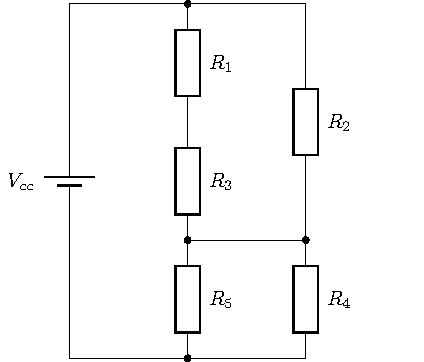
\includegraphics[scale=1.0]{fig-desafio}

      {\small Fonte: Próprio autor.}
    \end{figure}
  \end{minipage}
\end{minipage}
